\documentclass[a4paper,12pt]{article}

%%% HarrixLaTeXDocumentTemplate
%%% Версия 1.22
%%% Шаблон документов в LaTeX на русском языке. Данный шаблон применяется в проектах HarrixTestFunctions, MathHarrixLibrary, Standard-Genetic-Algorithm  и др.
%%% https://github.com/Harrix/HarrixLaTeXDocumentTemplate
%%% Шаблон распространяется по лицензии Apache License, Version 2.0.

%%% Проверка используемого TeX-движка %%%
\usepackage{ifxetex}

%%% Поля и разметка страницы %%%
\usepackage{lscape} % Для включения альбомных страниц
\usepackage{geometry} % Для последующего задания полей

%%% Кодировки и шрифты %%%
\ifxetex
\usepackage{polyglossia} % Поддержка многоязычности
\usepackage{fontspec} % TrueType-шрифты
\else
\usepackage{cmap}  % Улучшенный поиск русских слов в полученном pdf-файле
\usepackage[T2A]{fontenc} % Поддержка русских букв
\usepackage[utf8]{inputenc} % Кодировка utf8
\usepackage[english, russian]{babel} % Языки: русский, английский
\IfFileExists{pscyr.sty}{\usepackage{pscyr}}{} % Красивые русские шрифты
\fi

%%% Математические пакеты %%%
\usepackage{amsthm,amsfonts,amsmath,amssymb,amscd} % Математические дополнения от AMS
% Для жиного курсива в формулах %
\usepackage{bm}
% Для рисования некоторых математических символов (например, закрашенных треугольников)
\usepackage{mathabx}

%%% Оформление абзацев %%%
\usepackage{indentfirst} % Красная строка
\usepackage{setspace} % Расстояние между строками
\usepackage{enumitem} % Для список обнуление расстояния до абзаца

%%% Цвета %%%
\usepackage[usenames]{color}
\usepackage{color}
\usepackage{colortbl}

%%% Таблицы %%%
\usepackage{longtable} % Длинные таблицы
\usepackage{multirow,makecell,array} % Улучшенное форматирование таблиц

%%% Общее форматирование
\usepackage[singlelinecheck=off,center]{caption} % Многострочные подписи
\usepackage{soul} % Поддержка переносоустойчивых подчёркиваний и зачёркиваний
\usepackage{icomma} % Запятая в десятичных дробях

%%% Библиография %%%
\usepackage{cite}

%%% Гиперссылки %%%
\usepackage{hyperref}

%%% Изображения %%%
\usepackage{graphicx} % Подключаем пакет работы с графикой
\usepackage{epstopdf}
\usepackage{subcaption}

%%% Оглавление %%%
\usepackage{tocloft}

%%% Колонтитулы %%%
\usepackage{fancyhdr}

%%% Отображение кода %%%
\usepackage{xcolor}
\usepackage{listings}
\usepackage{caption}

%%% Псевдокоды %%%
\usepackage{algorithm} 
\usepackage{algpseudocode}

%%% Рисование графиков %%%
\usepackage{pgfplots}

%%% HarrixLaTeXDocumentTemplate
%%% Версия 1.22
%%% Шаблон документов в LaTeX на русском языке. Данный шаблон применяется в проектах HarrixTestFunctions, MathHarrixLibrary, Standard-Genetic-Algorithm  и др.
%%% https://github.com/Harrix/HarrixLaTeXDocumentTemplate
%%% Шаблон распространяется по лицензии Apache License, Version 2.0.

%%% Макет страницы %%%
% Выставляем значения полей (ГОСТ 7.0.11-2011, 5.3.7)
\geometry{a4paper,top=2cm,bottom=2cm,left=2.5cm,right=1cm}

%%% Выравнивание и переносы %%%
\sloppy % Избавляемся от переполнений
\clubpenalty=10000 % Запрещаем разрыв страницы после первой строки абзаца
\widowpenalty=10000 % Запрещаем разрыв страницы после последней строки абзаца


%%% Библиография %%%
\makeatletter
\bibliographystyle{utf8gost71u}  % Оформляем библиографию по ГОСТ 7.1 (ГОСТ Р 7.0.11-2011, 5.6.7)
\renewcommand{\@biblabel}[1]{#1.} % Заменяем библиографию с квадратных скобок на точку
\makeatother

%%% Изображения %%%
\graphicspath{{images/}} % Пути к изображениям
% Поменять двоеточние на точку в подписях к рисунку
\RequirePackage{caption}
\DeclareCaptionLabelSeparator{defffis}{. }
\captionsetup{justification=centering,labelsep=defffis}

%%% Абзацы %%%
% Отсупы между строками
\singlespacing
\setlength{\parskip}{0.3cm} % отступы между абзацами
\linespread{1.3} % Полуторный интвервал (ГОСТ Р 7.0.11-2011, 5.3.6)

% Оформление списков
\setlist{leftmargin=1.5cm,topsep=0pt}
% Используем дефис для ненумерованных списков (ГОСТ 2.105-95, 4.1.7)
\renewcommand{\labelitemi}{\normalfont\bfseries{--}}

%%% Цвета %%%
% Цвета для кода
\definecolor{string}{HTML}{B40000} % цвет строк в коде
\definecolor{comment}{HTML}{008000} % цвет комментариев в коде
\definecolor{keyword}{HTML}{1A00FF} % цвет ключевых слов в коде
\definecolor{morecomment}{HTML}{8000FF} % цвет include и других элементов в коде
\definecolor{сaptiontext}{HTML}{FFFFFF} % цвет текста заголовка в коде
\definecolor{сaptionbk}{HTML}{999999} % цвет фона заголовка в коде
\definecolor{bk}{HTML}{FFFFFF} % цвет фона в коде
\definecolor{frame}{HTML}{999999} % цвет рамки в коде
\definecolor{brackets}{HTML}{B40000} % цвет скобок в коде
% Цвета для гиперссылок
\definecolor{linkcolor}{HTML}{799B03} % цвет ссылок
\definecolor{urlcolor}{HTML}{799B03} % цвет гиперссылок
\definecolor{citecolor}{HTML}{799B03} % цвет гиперссылок
\definecolor{gray}{rgb}{0.4,0.4,0.4}
\definecolor{tableheadcolor}{HTML}{E5E5E5} % цвет шапки в таблицах
\definecolor{darkblue}{rgb}{0.0,0.0,0.6}
% Цвета для графиков
\definecolor{plotcoordinate}{HTML}{88969C}% цвет точек на координатых осях (минимум и максимум)
\definecolor{plotgrid}{HTML}{ECECEC} % цвет сетки
\definecolor{plotmain}{HTML}{97BBCD} % цвет основного графика
\definecolor{plotsecond}{HTML}{FF0000} % цвет второго графика, если графика только два
\definecolor{plotsecondgray}{HTML}{CCCCCC} % цвет второго графика, если графика только два. В сером виде.
\definecolor{darkgreen}{HTML}{799B03} % цвет темно-зеленого

%%% Отображение кода %%%
% Настройки отображения кода
\lstset{
language=C++, % Язык кода по умолчанию
morekeywords={*,...}, % если хотите добавить ключевые слова, то добавляйте
% Цвета
keywordstyle=\color{keyword}\ttfamily\bfseries,
%stringstyle=\color{string}\ttfamily,
stringstyle=\ttfamily\color{red!50!brown},
commentstyle=\color{comment}\ttfamily\itshape,
morecomment=[l][\color{morecomment}]{\#}, 
% Настройки отображения     
breaklines=true, % Перенос длинных строк
basicstyle=\ttfamily\footnotesize, % Шрифт для отображения кода
backgroundcolor=\color{bk}, % Цвет фона кода
frame=lrb,xleftmargin=\fboxsep,xrightmargin=-\fboxsep, % Рамка, подогнанная к заголовку
rulecolor=\color{frame}, % Цвет рамки
tabsize=3, % Размер табуляции в пробелах
% Настройка отображения номеров строк. Если не нужно, то удалите весь блок
%numbers=left, % Слева отображаются номера строк
%stepnumber=1, % Каждую строку нумеровать
%numbersep=5pt, % Отступ от кода 
%numberstyle=\small\color{black}, % Стиль написания номеров строк
% Для отображения русского языка
extendedchars=true,
literate={Ö}{{\"O}}1
  {Ä}{{\"A}}1
  {Ü}{{\"U}}1
  {ß}{{\ss}}1
  {ü}{{\"u}}1
  {ä}{{\"a}}1
  {ö}{{\"o}}1
  {~}{{\textasciitilde}}1
  {а}{{\selectfont\char224}}1
  {б}{{\selectfont\char225}}1
  {в}{{\selectfont\char226}}1
  {г}{{\selectfont\char227}}1
  {д}{{\selectfont\char228}}1
  {е}{{\selectfont\char229}}1
  {ё}{{\"e}}1
  {ж}{{\selectfont\char230}}1
  {з}{{\selectfont\char231}}1
  {и}{{\selectfont\char232}}1
  {й}{{\selectfont\char233}}1
  {к}{{\selectfont\char234}}1
  {л}{{\selectfont\char235}}1
  {м}{{\selectfont\char236}}1
  {н}{{\selectfont\char237}}1
  {о}{{\selectfont\char238}}1
  {п}{{\selectfont\char239}}1
  {р}{{\selectfont\char240}}1
  {с}{{\selectfont\char241}}1
  {т}{{\selectfont\char242}}1
  {у}{{\selectfont\char243}}1
  {ф}{{\selectfont\char244}}1
  {х}{{\selectfont\char245}}1
  {ц}{{\selectfont\char246}}1
  {ч}{{\selectfont\char247}}1
  {ш}{{\selectfont\char248}}1
  {щ}{{\selectfont\char249}}1
  {ъ}{{\selectfont\char250}}1
  {ы}{{\selectfont\char251}}1
  {ь}{{\selectfont\char252}}1
  {э}{{\selectfont\char253}}1
  {ю}{{\selectfont\char254}}1
  {я}{{\selectfont\char255}}1
  {А}{{\selectfont\char192}}1
  {Б}{{\selectfont\char193}}1
  {В}{{\selectfont\char194}}1
  {Г}{{\selectfont\char195}}1
  {Д}{{\selectfont\char196}}1
  {Е}{{\selectfont\char197}}1
  {Ё}{{\"E}}1
  {Ж}{{\selectfont\char198}}1
  {З}{{\selectfont\char199}}1
  {И}{{\selectfont\char200}}1
  {Й}{{\selectfont\char201}}1
  {К}{{\selectfont\char202}}1
  {Л}{{\selectfont\char203}}1
  {М}{{\selectfont\char204}}1
  {Н}{{\selectfont\char205}}1
  {О}{{\selectfont\char206}}1
  {П}{{\selectfont\char207}}1
  {Р}{{\selectfont\char208}}1
  {С}{{\selectfont\char209}}1
  {Т}{{\selectfont\char210}}1
  {У}{{\selectfont\char211}}1
  {Ф}{{\selectfont\char212}}1
  {Х}{{\selectfont\char213}}1
  {Ц}{{\selectfont\char214}}1
  {Ч}{{\selectfont\char215}}1
  {Ш}{{\selectfont\char216}}1
  {Щ}{{\selectfont\char217}}1
  {Ъ}{{\selectfont\char218}}1
  {Ы}{{\selectfont\char219}}1
  {Ь}{{\selectfont\char220}}1
  {Э}{{\selectfont\char221}}1
  {Ю}{{\selectfont\char222}}1
  {Я}{{\selectfont\char223}}1
  {і}{{\selectfont\char105}}1
  {ї}{{\selectfont\char168}}1
  {є}{{\selectfont\char185}}1
  {ґ}{{\selectfont\char160}}1
  {І}{{\selectfont\char73}}1
  {Ї}{{\selectfont\char136}}1
  {Є}{{\selectfont\char153}}1
  {Ґ}{{\selectfont\char128}}1
  {\{}{{{\color{brackets}\{}}}1 % Цвет скобок {
  {\}}{{{\color{brackets}\}}}}1 % Цвет скобок }
}
% Для настройки заголовка кода
\DeclareCaptionFont{white}{\color{сaptiontext}}
\DeclareCaptionFormat{listing}{\parbox{\linewidth}{\colorbox{сaptionbk}{\parbox{\linewidth}{#1#2#3}}\vskip-4pt}}
\captionsetup[lstlisting]{format=listing,labelfont=white,textfont=white}
\renewcommand{\lstlistingname}{Код} % Переименование Listings в нужное именование структуры
% Для отображения кода формата xml
\lstdefinelanguage{XML}
{
  morestring=[s]{"}{"},
  morecomment=[s]{?}{?},
  morecomment=[s]{!--}{--},
  commentstyle=\color{comment},
  moredelim=[s][\color{black}]{>}{<},
  moredelim=[s][\color{red}]{\ }{=},
  stringstyle=\color{string},
  identifierstyle=\color{keyword}
}

%%% Гиперссылки %%%
\hypersetup{pdfstartview=FitH,  linkcolor=linkcolor,urlcolor=urlcolor,citecolor=citecolor, colorlinks=true}

%%% Псевдокоды %%%
% Добавляем свои блоки
\makeatletter
\algblock[ALGORITHMBLOCK]{BeginAlgorithm}{EndAlgorithm}
\algblock[BLOCK]{BeginBlock}{EndBlock}
\makeatother

% Нумерация блоков
\usepackage{caption}% http://ctan.org/pkg/caption
\captionsetup[ruled]{labelsep=period}
\makeatletter
\@addtoreset{algorithm}{chapter}% algorithm counter resets every chapter
\makeatother
\renewcommand{\thealgorithm}{\thechapter.\arabic{algorithm}}% Algorithm # is <chapter>.<algorithm>

%%% Формулы %%%
%Дублирование символа при переносе
\newcommand{\hmm}[1]{#1\nobreak\discretionary{}{\hbox{\ensuremath{#1}}}{}}

%%% Таблицы %%%
% Раздвигаем в таблице без границ отступы между строками в новой команде
\newenvironment{tabularwide}%
{\setlength{\extrarowheight}{0.3cm}\begin{tabular}{  p{\dimexpr 0.45\linewidth-2\tabcolsep} p{\dimexpr 0.55\linewidth-2\tabcolsep}  }}  {\end{tabular}}
\newenvironment{tabularwide08}%
{\setlength{\extrarowheight}{0.3cm}\begin{tabular}{  p{\dimexpr 0.8\linewidth-2\tabcolsep} p{\dimexpr 0.2\linewidth-2\tabcolsep}  }}  {\end{tabular}}

% Многострочная ячейка в таблице
\newcommand{\specialcell}[2][c]{%
  {\renewcommand{\arraystretch}{1}\begin{tabular}[t]{@{}l@{}}#2\end{tabular}}}

% Многострочная ячейка, где текст не может выйти за границы
\newcolumntype{P}[1]{>{\raggedright\arraybackslash}p{#1}}
\newcommand{\specialcelltwoin}[2][c]{%
  {\renewcommand{\arraystretch}{1}\begin{tabular}[t]{@{}P{1.98in}@{}}#2\end{tabular}}}
  
% Команда для переворачивания текста в ячейке таблицы на 90 градусов
\newcommand*\rot{\rotatebox{90}}

%%% Рисование графиков %%%
\pgfplotsset{
every axis legend/.append style={at={(0.5,-0.13)},anchor=north,legend cell align=left},
tick label style={font=\tiny\scriptsize},
label style={font=\scriptsize},
legend style={font=\scriptsize},
grid=both,
minor tick num=2,
major grid style={plotgrid},
minor grid style={plotgrid},
axis lines=left,
legend style={draw=none},
/pgf/number format/.cd,
1000 sep={}
}
% Карта цвета для трехмерных графиков в стиле графиков Mathcad
\pgfplotsset{
/pgfplots/colormap={mathcad}{rgb255(0cm)=(76,0,128) rgb255(2cm)=(0,14,147) rgb255(4cm)=(0,173,171) rgb255(6cm)=(32,205,0) rgb255(8cm)=(229,222,0) rgb255(10cm)=(255,13,0)}
}
% Карта цвета для трехмерных графиков в стиле графиков Matlab
\pgfplotsset{
/pgfplots/colormap={matlab}{rgb255(0cm)=(0,0,128) rgb255(1cm)=(0,0,255) rgb255(3cm)=(0,255,255) rgb255(5cm)=(255,255,0) rgb255(7cm)=(255,0,0) rgb255(8cm)=(128,0,0)}
}

%%% Разное %%%
% Галочки для отмечания в тескте вариантов как OK
\def\checkmark{\tikz\fill[black,scale=0.3](0,.35) -- (.25,0) -- (1,.7) -- (.25,.15) -- cycle;}
\def\checkmarkgreen{\tikz\fill[darkgreen,scale=0.3](0,.35) -- (.25,0) -- (1,.7) -- (.25,.15) -- cycle;} 
\def\checkmarkred{\tikz\fill[red,scale=0.3](0,.35) -- (.25,0) -- (1,.7) -- (.25,.15) -- cycle;}
\def\checkmarkbig{\tikz\fill[black,scale=0.5](0,.35) -- (.25,0) -- (1,.7) -- (.25,.15) -- cycle;}
\def\checkmarkbiggreen{\tikz\fill[darkgreen,scale=0.5](0,.35) -- (.25,0) -- (1,.7) -- (.25,.15) -- cycle;} 
\def\checkmarkbigred{\tikz\fill[red,scale=0.5](0,.35) -- (.25,0) -- (1,.7) -- (.25,.15) -- cycle;}

%% Следующие блоки расскоментировать при необходимости

%%% Кодировки и шрифты %%%
%\ifxetex
%\setmainlanguage{russian}
%\setotherlanguage{english}
%\defaultfontfeatures{Ligatures=TeX,Mapping=tex-text}
%\setmainfont{Times New Roman}
%\newfontfamily\cyrillicfont{Times New Roman}
%\setsansfont{Arial}
%\newfontfamily\cyrillicfontsf{Arial}
%\setmonofont{Courier New}
%\newfontfamily\cyrillicfonttt{Courier New}
%\else
%\IfFileExists{pscyr.sty}{\renewcommand{\rmdefault}{ftm}}{}
%\fi

%%% Колонтитулы %%%
% Порядковый номер страницы печатают на середине верхнего поля страницы (ГОСТ Р 7.0.11-2011, 5.3.8)
%\makeatletter
%\let\ps@plain\ps@fancy              % Подчиняем первые страницы каждой главы общим правилам
%\makeatother
%\pagestyle{fancy}                   % Меняем стиль оформления страниц
%\fancyhf{}                          % Очищаем текущие значения
%\fancyhead[C]{\thepage}             % Печатаем номер страницы на середине верхнего поля
%\renewcommand{\headrulewidth}{0pt}  % Убираем разделительную линию

%%% Оглавление %%%
%\renewcommand{\cftchapdotsep}{\cftdotsep}
%\renewcommand{\cftchapleader}{\cftdotfill{\cftdotsep}}
%\renewcommand{\cftsecleader}{\cftdotfill{\cftdotsep}}
%\renewcommand{\cftfigleader}{\cftdotfill{\cftdotsep}}
%\renewcommand{\cfttableader}{\cftdotfill{\cftdotsep}}

\title{HarrixMakeLibrary v.1.7}
\author{А.\,Б. Сергиенко}
\date{\today}


\begin{document}

%%% HarrixLaTeXDocumentTemplate
%%% Версия 1.22
%%% Шаблон документов в LaTeX на русском языке. Данный шаблон применяется в проектах HarrixTestFunctions, MathHarrixLibrary, Standard-Genetic-Algorithm  и др.
%%% https://github.com/Harrix/HarrixLaTeXDocumentTemplate
%%% Шаблон распространяется по лицензии Apache License, Version 2.0.

%%% Именования %%%
\renewcommand{\abstractname}{Аннотация}
\renewcommand{\alsoname}{см. также}
\renewcommand{\appendixname}{Приложение} % (ГОСТ Р 7.0.11-2011, 5.7)
\renewcommand{\bibname}{Список литературы} % (ГОСТ Р 7.0.11-2011, 4)
\renewcommand{\ccname}{исх.}
\renewcommand{\chaptername}{Глава}
\renewcommand{\contentsname}{Оглавление} % (ГОСТ Р 7.0.11-2011, 4)
\renewcommand{\enclname}{вкл.}
\renewcommand{\figurename}{Рисунок} % (ГОСТ Р 7.0.11-2011, 5.3.9)
\renewcommand{\headtoname}{вх.}
\renewcommand{\indexname}{Предметный указатель}
\renewcommand{\listfigurename}{Список рисунков}
\renewcommand{\listtablename}{Список таблиц}
\renewcommand{\pagename}{Стр.}
\renewcommand{\partname}{Часть}
\renewcommand{\refname}{Список литературы} % (ГОСТ Р 7.0.11-2011, 4)
\renewcommand{\seename}{см.}
\renewcommand{\tablename}{Таблица} % (ГОСТ Р 7.0.11-2011, 5.3.10)

%%% Псевдокоды %%%
% Перевод данных об алгоритмах
\renewcommand{\listalgorithmname}{Список алгоритмов}
\floatname{algorithm}{Алгоритм}

% Перевод команд псевдокода
\algrenewcommand\algorithmicwhile{\textbf{До тех пока}}
\algrenewcommand\algorithmicdo{\textbf{выполнять}}
\algrenewcommand\algorithmicrepeat{\textbf{Повторять}}
\algrenewcommand\algorithmicuntil{\textbf{Пока выполняется}}
\algrenewcommand\algorithmicend{\textbf{Конец}}
\algrenewcommand\algorithmicif{\textbf{Если}}
\algrenewcommand\algorithmicelse{\textbf{иначе}}
\algrenewcommand\algorithmicthen{\textbf{тогда}}
\algrenewcommand\algorithmicfor{\textbf{Цикл. }}
\algrenewcommand\algorithmicforall{\textbf{Выполнить для всех}}
\algrenewcommand\algorithmicfunction{\textbf{Функция}}
\algrenewcommand\algorithmicprocedure{\textbf{Процедура}}
\algrenewcommand\algorithmicloop{\textbf{Зациклить}}
\algrenewcommand\algorithmicrequire{\textbf{Условия:}}
\algrenewcommand\algorithmicensure{\textbf{Обеспечивающие условия:}}
\algrenewcommand\algorithmicreturn{\textbf{Возвратить}}
\algrenewtext{EndWhile}{\textbf{Конец цикла}}
\algrenewtext{EndLoop}{\textbf{Конец зацикливания}}
\algrenewtext{EndFor}{\textbf{Конец цикла}}
\algrenewtext{EndFunction}{\textbf{Конец функции}}
\algrenewtext{EndProcedure}{\textbf{Конец процедуры}}
\algrenewtext{EndIf}{\textbf{Конец условия}}
\algrenewtext{EndFor}{\textbf{Конец цикла}}
\algrenewtext{BeginAlgorithm}{\textbf{Начало алгоритма}}
\algrenewtext{EndAlgorithm}{\textbf{Конец алгоритма}}
\algrenewtext{BeginBlock}{\textbf{Начало блока. }}
\algrenewtext{EndBlock}{\textbf{Конец блока}}
\algrenewtext{ElsIf}{\textbf{иначе если }}

\maketitle

\begin{abstract}
\textbf{HarrixMakeLibrary} --- это программа собирающая библиотеки функций на языке C++ и справку к ним из исходных материалов.
\end{abstract}

\tableofcontents

\newpage

\section{Внешний вид программы}

\begin{figure} [h] 
  \center
  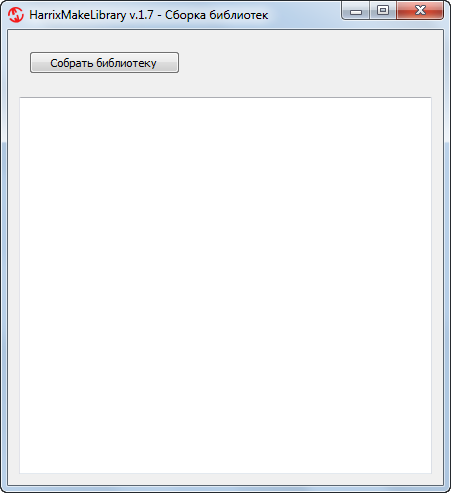
\includegraphics [scale=0.5] {makemainwindow.png}
  \caption{Внешний вид программы} 
  \label{img:latex}  
\end{figure}

При нажатии на кнопку \textbf{<<Собрать библиотеку>>} будет производиться сборка библиотеки вместе с файлами справки. После чего будет открыта папка с сформированными файлами.

В текстовом поле под кнопкой будет отображаться ход работы программы.

Это программа является упрощенной версией программы \textbf{MakeHarrixMathLibrary} из библиотеки \textbf{HarrixMathLibrary}. Помогает собирать файлы библиотек, если каждая функция прописана в отдельных файлах.

\section{Результат работы программы}

В папке \textbf{source\_library} находится исходный материал, который обрабатывается программой HarrixMakeLibrary.exe, в результате чего образуются следующие элементы:

\begin{itemize}
\item \textbf{Library.cpp} --- главный файл библиотеки;
\item \textbf{Library.h} --- заголовочный файл;
\item \textbf{Library\_Help.tex} --- файл справки в формате \LaTeX.
\end{itemize}

Обратите внимание, что это не полноценные файлы исходников библиотеки --- это только сборка функций в соответствующие файлы. И код этих файлов надо вставлять в ваши основные файлы исходных кодов библиотек. В общем, программа генерирует основу, а всякие дополнительные элементы вроде подключение include и др. это вам самим прописывать.

Все данные файлы собираются в папке \textbf{temp\_library}.

\section{Как собирается библиотека}
Исходники библиотеки находятся с папке \textbf{source\_library}.

Файлы \textbf{Library.cpp} и \textbf{Library.h} собираются следующим образом.

В папке \textbf{source\_library} есть директории. Каждая директория --- это множество функций какого-то раздела. Перед рассмотрением файлов папки программа добавляет в файл Library.cpp следующий код:

\begin{lstlisting}[label=make_sectioncpp,caption=Название раздела]
//*****************************************************************
//[Название папки]
//*****************************************************************
\end{lstlisting}

А в файл Library.h добавляется код:

\begin{lstlisting}[label=make_sectionh,caption=Название раздела]
//[Название папки]
\end{lstlisting}

После каждой функции в Library.cpp вставляется код:
\begin{lstlisting}[label=make_sectionh,caption=Название раздела]
//---------------------------------------------------------------------------
\end{lstlisting}

Далее программа пробегает по каждой папке, которая представляет собой раздел функций в библиотеке. Каждая функция в разделе предоставляется следующими файлами:
\begin{itemize}
\item \textbf{<File>.cpp} или \textbf{<File>.tpp} --- код функции;
\item \textbf{<File>.h} --- заголовочный файл функции;
\item \textbf{<File>.tex} --- справка по функции;
\item \textbf{<File>.desc} --- описание функции;
\item \textbf{<File>.use} --- пример использования функции (из него удаляются пробелы в начале строк, равным числу пробелов вначале первой строки);
\item \textbf{<File>\_<name>.pdf} --- множество рисунков, необходимых для справки по функции (необязательные файлы);
\item \textbf{<File>\_<name>.png} --- множество рисунков, необходимых для справки по функции (необязательные файлы);
\end{itemize}

Важно помнить, что каждый *.cpp, *.h, *.tex файл в папках папки \textbf{source\_library} не является полноценным файлом соответствующего расширения и без сборки в единые файлы библиотеки не может использоваться.

Разница файлов *.cpp и *.tpp в том, что в *.tpp  пишется код шаблонов функций, а в *.cpp пишутся обычные функции, и их реализация располагается в Library.cpp файле, тогда как шаблоны располагаются в Library.h файле.

Ниже показан алгоритм (Алгоритм \ref{alg:MakingCppH}) формирования файлов библиотеки.

Итоговое количество функций определяется как количество знаков <<;>> в h файлах функций, которые располагаются в папках.


\begin{algorithm}
\caption{Алгоритм собирания файлов библиотеки} \label{alg:MakingCppH}
\begin{algorithmic}
\State \textbf{Начало алгоритма}
\ForAll {папок}
\State $ Library.cpp+=\text{\textit{Код 1. Название раздела}} $;
\State $ Library.h+=\text{\textit{Код 2. Название раздела}} $;
\ForAll {файлов папки расширения *.cpp, *.tpp и *.h}
\If {есть файл *.cpp}
\State $ Library.cpp+=<File>.cpp $;
\Else
\State $ ResultTpp+=<File>.tpp $;
\EndIf
\State $ Library.h+=<File>.h $;
\EndFor
\EndFor
\State $ Library.h+= ResultTpp$;
\State Сохранить $ Library.cpp $ в папке temp\_library;
\State Сохранить $ Library.h $ в папке temp\_library;
\State \textbf{Конец алгоритма}
\end{algorithmic}
\end{algorithm}

Стоит отметить, что все разделы функций и сами функции сортируются в алфавитном порядке.


\section{Как собирается справка}
Исходники файлов справки библиотеки находятся с папке
\textbf{source\_library}.

Файлы \textbf{Library.tex} собирается следующим образом, как показано ниже в алгоритме (Алгоритм \ref{alg:MakingHelp}) формирования файлов справки библиотеки.

Некоторые моменты по преобразованию некоторых данных (например, преобразование $<File>.desc$) не рассматривается в алгоритме, но вы можете все посмотреть в исходном коде программы, которая поставляется с данной библиотекой в папке \textbf{source\textbackslash}

Также еще собирается файл \textbf{FUNCTIONS.md} со списком функций в формате \textbf{Markdown}, например, для размещения в GitHub.

\section{Исходники HarrixMakeLibrary.exe и справки по ним}

HarrixMakeLibrary написан на Qt.  Не требует каких-то дополнительных файлов. Исходники программы располагаются в папке \textbf{source\textbackslash}.

Исходники справки HarrixMakeLibrary (данного файла, который вы читаете) по располагаются в папке \textbf{source\textbackslash help\textbackslash}. Главный файл исходника справки --- это файл HarrixMakeLibrary\_Help.tex.

\begin{algorithm}
\caption{Алгоритм собирания файлов справки библиотеки} \label{alg:MakingHelp}
\begin{algorithmic}
\State \textbf{Начало алгоритма}
\State $ResultTexList += \text {\textit{Заголовок для списка функций}}$;
\State $ResultTexFunctions += \text {\textit{Заголовок для функций}}$;
\ForAll {папок}
\State $ ResultTexList+=\text{\textit{Заголовок раздела}} $;
\State $ ResultTexFunctions+=\text{\textit{Заголовок раздела}} $;
\State $n=0$;
\ForAll {файлов папки расширения *.desc, *.tex, *.h, *.use}
\State $ ResultTexList+=<File>.desc $ в обработке;
\State $ ResultTexFunctions+=<File>.desc $ в обработке;
\State $ ResultTexFunctions+=<File>.h $ в обертке;
\State $ ResultTexFunctions+=<File>.tex $;
\State $ ResultTexFunctions+=<File>.use $ в обертке;
\State $n++$;
\EndFor
\ForAll {файлов папки расширения *.pdf и *.png}
\State  Скопировать файл <File>.<png|pdf> в папку \textbf{\textbackslash images\textbackslash};
\EndFor
\EndFor
\State $ Library\_Help.tex+=ResultTexList $;
\State $ Library\_Help.tex+=ResultTexFunctions $;
\State Сохранить $ Library\_Help.tex $ в папке temp\_library;
\State \textbf{Конец алгоритма}
\end{algorithmic}
\end{algorithm}

\end{document}
